\begin{figure}[htb]
    \centering
    
\includegraphics[width=0.75\columnwidth]{HTML5logos}
    \caption{Official HTML5 logo \& unofficial CSS3 logo.}
    \label{fig:html-logos}
\end{figure}

When speaking of \ac{HTML}5 one, usually, is not only focusing on the markup language
but on a set of web technologies and specifications strictly related to \ac{HTML}5.
This set of technologies includes the \ac{HTML}5 specification itself, the
\ac{CSS}3 recommendations and a whole new set of \js{} APIs. So, first things
first, let us point out the differences:
\begin{description}
	\item[HTML5] refers to a set of semantic tags (like \ctag{footer},
	\ctag{header}, \ctag{article}, \ldots), media tags (like \ctag{video} or
	\ctag{audio}) and the so called Web Form 2.0 alongside with all the "old"
	tags inherited from HTML4. These tags help developers to give semantics to
	the website they make, so the websites can be
	better understood by search engines or HTML parsers (like those used for
	reading the site for blind people).

	\item[CSS3] refers to the presentation layer of the pages. Here are introduced
	specifications including image effects, 3D transformation, new tag selectors, 
	form element validation, etc. The specifications take care also of the new
	devices (like smartphones and tablets) giving the user the \code{media
	queries} to examine the media (screen, print, aural) and provide different
	\ac{CSS} rules.
	
	\item[JS] refers to the \js{} with a new set of API for interacting with the
	new media elements and other tags, as long as API for concurrent computation,
	real-time communication, offline storage, etc.\\
\end{description}

With the advent of \ac{HTML}5, like any new technology, many problems were
resolved and many others have been created. The main issue with using \ac{HTML}5
is the browser compatibility and browser-specific methods.

When browsers start
implementing some \ac{HTML}5 draft feature, since they are not fully standardized
\footnote{In fact HTML5 (at the time of writing) is not yet standardized, its
still a draft. See \url{http://www.w3.org/TR/html5/}}, they prevent the pollution
of the DOM by prefixing the standard method
with a browser specific prefix\footnote{\code{o}: for
Opera, \code{ms}: for Internet Explorer, \code{moz}: for Firefox, and
\code{webkit}: for the WebKit based browser (Chrome and Safari)}(i.e.
\linebreak\code{requestAnimFrame}
can become \code{mozRequestAnimFrame} or \code{webkitRequestAnimFrame}). This prefixing
is particularly common in the \ac{CSS}3 where things becomes awful\footnote{See
CSS animation or gradients for example.}.\\


To avoid browser inconsistency there are plenty of \js{} frameworks for every
purpose. Frameworks like \citetitle{jquery} provide a layer of abstraction between
browser-specific code and the user, giving developers fallbacks for the most
common API and additional features not covered by the standard implementation.
Other frameworks like \citetitle{modernizr} give developers the ability to test
if some \ac{HTML}5 feature is available in the currently used browser and provide
a general fallback system for dynamically load polyfills\footnote{A polyfill is
a \js{} library or third part plugin that emulates one or more HTML5 feature,
providing websites to have a consistent behavior.}.\\


Now are presented the main \ac{HTML}5 features to better understand how they can
be used in this System.





\paragraph{Canvas}
Let's start with the official definition\footnote{Got from the specs:
\url{http://www.w3.org/TR/html5/the-canvas-element.html\#the-canvas-element}}
\begin{quoting}\rm\tt
	The canvas element provides scripts with a resolution-dependent bitmap canvas, which can
	be used for rendering graphs, game graphics, or other visual images on the fly.
\end{quoting}

So the \code{canvas} element is basically a \emph{Canvas}, like the name says, where
one can \emph{paint} anything. On top of this, the \code{canvas} element gives
the developers access to the underlying raw pixel data. Also in the \code{canvas}
element you can \emph{draw} images taken from a \ctag{img} tag or a frame taken
from a \ctag{video} tag.

As one can see now we have all the tools we need to perform image analysis or
video manipulation within the browser. Obviously there are plenty of \js{}
libraries that facilitate the whole process of filtering or, in general, image
manipulation (like \href{http://www.pixastic.com/}{Pixastic} or
\href{http://camanjs.com/}{Camanjs}). Other libraries give you the tools to
create diagrams or charts on the fly (like \href{http://raphaeljs.com/}{Raphaël}
or \href{http://processingjs.org/}{Processingjs}).

The canvas element also provides a 3D context to draw and animate
\footnote{Animations are not natively supported, must be coded separately.}
high definition graphics and models using the WebGL API. This API is maintained
by the \href{http://www.khronos.org/}{Khronos Group} and is based on OpenGL ES
2.0 specifications. On top of these API there are a lot of libraries\footnote{For
a reference see \url{http://en.wikipedia.org/wiki/WebGL\#Developer_libraries}}
made to facilitate development of 3D applications. One of the the most used is
the \href{http://mrdoob.github.com/three.js/}{Three} \js{} library, that can be
used for creating and animating 2D or 3D scenes within the canvas element.








\paragraph{WebSocket}
The WebSocket is an API interface for enabling bi-directional full-duplex client
server communication on top of the \ac{TCP}. It enables real-time
communication between clients and servers, allowing servers to \textbf{push} data
to the clients and obtain \emph{real} real-time content updates.

Like many other \ac{HTML}5 features on top of WebSocket a library that
provides easy access to these functionality as long as fallbacks for old browsers
was built.
\citetitle{socket.io} provides a single entry-point to create a connection to the
server and manage the message exchange, providing fallbacks\footnote{If WebSocket,
are not available the library can use Adobe\reg Flash\reg Socket, AJAX long
polling, AJAX multi-part streaming, Forever Iframe and JSONP Polling} to ensure
cross-browser compatibility.





\paragraph{WebWorkers}\label{html5:workers}
A problem that rises when coding load intensive \js{} application is the single thread nature
of the language. Every script runs in the same thread of the browser window/tab.
This can lead to some unwanted behavior (like browser freezing or a warning
dialog that that alerts the user as in \autoref{fig:browser-slow-dialog}).
\begin{figure}[htb]
    \centering
    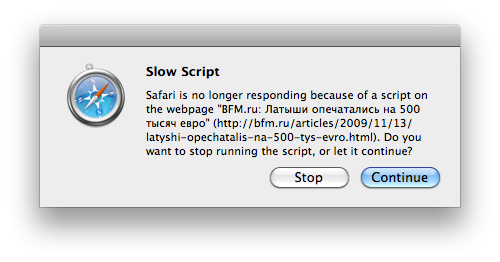
\includegraphics[width=0.75\columnwidth]{browser-slow-dialog}
    \caption{The slow script dialog.}
    \label{fig:browser-slow-dialog}
\end{figure}
To solve this problem \cite{jenkin2008parasitic} proposed a timed-based
programming structure that ensures that the code runs without any browser warning
or freezing and also offers the developer to tweak the performance of the script
by dynamically adjusting the interval between the step execution. This method
leverage on the \code{setTimeout} function of \js{} in order to split code into
timestep-driven code chunks to execute. Here is an example of loop translated
into a timer-based loop:
\begin{multicols}{2}
	\begin{algorithm}[H]
		\While{condition}{
			...do something...
		}
	\end{algorithm}

	\vfill
	\columnbreak

	\begin{algorithm}[H]
		\SetKwBlock{procedure}{procedure}{}
		\SetKwFunction{setTimeout}{setTimeout}

		\procedure(STEP){
			...do something...\\
			\If{condition}{
				\setTimeout{STEP, delay}
			}
		}
	\end{algorithm}
\end{multicols}
Obviously this is not the solution to the problem, it is a hack that tricks the
browser.\\


WebWorkers offer a simpler solution. They provide a simple, yet powerful, way of
creating \emph{threads} in \js{}. The official definition says:
\begin{quoting}\rm\tt
	The WebWorkers specification defines an API for running scripts in the
	background independently of any user interface scripts.	This allows for
	long-running scripts that are not interrupted by scripts that respond to
	clicks or other user interactions, and allows long tasks to be executed
	without yielding to keep the page responsive.
\end{quoting}

The core concept behind WebWorkers is the \code{Worker}. A \code{Worker} is a
piece of \js{} code that runs in parallel to the main thread and is able to send
and receive messages (just like normal threads).



\paragraph{Storage}
When web developers think of storing anything about the user, they immediately
think of uploading to the server. \ac{HTML}5 changes that, as there are now
several technologies allowing the \ac{RIA} to save data on the client device.

\ac{HTML}5 supports a number of storage techniques able to store data within the
browser to be accessed later. Here is a simple list with the principal features:
\begin{description}
	\item[Web storage] is a convenient form for offline storage. It uses a simple
	key-value mapping for storing data persistently on the browser.

	\item[Web SQL database] is an offline SQL database, usually implemented using
	SQLite, a general-purpose open-source SQL engine.

	\item[IndexedDB] is a nice compromise between Web Storage and Web SQL Database.
	Like the former, it is relatively simple and like the latter, it's capable
	of being very fast. It uses the same mapping as \emph{Web storage} and indexes
	certain fields inside the stored data.

	\item[Filesystem API], as the name says, offers the ability to manipulate the
	file system of the host.
\end{description}


\paragraph{Offline storage}
In this category falls the \code{application cache}. The \code{application cache} is
controlled by a plain text file called a \code{manifest}, which contains a list
of resources to be stored for use when there is no network connectivity. The list
can also define the conditions for caching, such as which pages should never be
cached and even what to show the user when he follows a link to an uncached page.

If the user goes offline but has visited the site while online, the cached
resources will be loaded so the user can still view the site in a limited form.
Here is a simple cache file:
\begin{lstlisting}[language=make]
CACHE MANIFEST
      
# This is a comment

CACHE:
/css/screen.css
/css/offline.css
/js/screen.js
/img/logo.png

http://example.com/css/styles.css

FALLBACK:
/ /offline.html

NETWORK:
*
\end{lstlisting}